\documentclass[
  man,
  floatsintext,
  longtable,
  nolmodern,
  notxfonts,
  notimes,
  colorlinks=true,linkcolor=blue,citecolor=blue,urlcolor=blue]{apa7}

\usepackage{amsmath}
\usepackage{amssymb}




\RequirePackage{longtable}
\RequirePackage{threeparttablex}

\makeatletter
\renewcommand{\paragraph}{\@startsection{paragraph}{4}{\parindent}%
	{0\baselineskip \@plus 0.2ex \@minus 0.2ex}%
	{-.5em}%
	{\normalfont\normalsize\bfseries\typesectitle}}

\renewcommand{\subparagraph}[1]{\@startsection{subparagraph}{5}{0.5em}%
	{0\baselineskip \@plus 0.2ex \@minus 0.2ex}%
	{-\z@\relax}%
	{\normalfont\normalsize\bfseries\itshape\hspace{\parindent}{#1}\textit{\addperi}}{\relax}}
\makeatother




\usepackage{longtable, booktabs, multirow, multicol, colortbl, hhline, caption, array, float, xpatch}
\setcounter{topnumber}{2}
\setcounter{bottomnumber}{2}
\setcounter{totalnumber}{4}
\renewcommand{\topfraction}{0.85}
\renewcommand{\bottomfraction}{0.85}
\renewcommand{\textfraction}{0.15}
\renewcommand{\floatpagefraction}{0.7}

\usepackage{tcolorbox}
\tcbuselibrary{listings,theorems, breakable, skins}
\usepackage{fontawesome5}

\definecolor{quarto-callout-color}{HTML}{909090}
\definecolor{quarto-callout-note-color}{HTML}{0758E5}
\definecolor{quarto-callout-important-color}{HTML}{CC1914}
\definecolor{quarto-callout-warning-color}{HTML}{EB9113}
\definecolor{quarto-callout-tip-color}{HTML}{00A047}
\definecolor{quarto-callout-caution-color}{HTML}{FC5300}
\definecolor{quarto-callout-color-frame}{HTML}{ACACAC}
\definecolor{quarto-callout-note-color-frame}{HTML}{4582EC}
\definecolor{quarto-callout-important-color-frame}{HTML}{D9534F}
\definecolor{quarto-callout-warning-color-frame}{HTML}{F0AD4E}
\definecolor{quarto-callout-tip-color-frame}{HTML}{02B875}
\definecolor{quarto-callout-caution-color-frame}{HTML}{FD7E14}

%\newlength\Oldarrayrulewidth
%\newlength\Oldtabcolsep


\usepackage{hyperref}




\providecommand{\tightlist}{%
  \setlength{\itemsep}{0pt}\setlength{\parskip}{0pt}}
\usepackage{longtable,booktabs,array}
\usepackage{calc} % for calculating minipage widths
% Correct order of tables after \paragraph or \subparagraph
\usepackage{etoolbox}
\makeatletter
\patchcmd\longtable{\par}{\if@noskipsec\mbox{}\fi\par}{}{}
\makeatother
% Allow footnotes in longtable head/foot
\IfFileExists{footnotehyper.sty}{\usepackage{footnotehyper}}{\usepackage{footnote}}
\makesavenoteenv{longtable}

\usepackage{graphicx}
\makeatletter
\def\maxwidth{\ifdim\Gin@nat@width>\linewidth\linewidth\else\Gin@nat@width\fi}
\def\maxheight{\ifdim\Gin@nat@height>\textheight\textheight\else\Gin@nat@height\fi}
\makeatother
% Scale images if necessary, so that they will not overflow the page
% margins by default, and it is still possible to overwrite the defaults
% using explicit options in \includegraphics[width, height, ...]{}
\setkeys{Gin}{width=\maxwidth,height=\maxheight,keepaspectratio}
% Set default figure placement to htbp
\makeatletter
\def\fps@figure{htbp}
\makeatother


% definitions for citeproc citations
\NewDocumentCommand\citeproctext{}{}
\NewDocumentCommand\citeproc{mm}{%
  \begingroup\def\citeproctext{#2}\cite{#1}\endgroup}
\makeatletter
 % allow citations to break across lines
 \let\@cite@ofmt\@firstofone
 % avoid brackets around text for \cite:
 \def\@biblabel#1{}
 \def\@cite#1#2{{#1\if@tempswa , #2\fi}}
\makeatother
\newlength{\cslhangindent}
\setlength{\cslhangindent}{1.5em}
\newlength{\csllabelwidth}
\setlength{\csllabelwidth}{3em}
\newenvironment{CSLReferences}[2] % #1 hanging-indent, #2 entry-spacing
 {\begin{list}{}{%
  \setlength{\itemindent}{0pt}
  \setlength{\leftmargin}{0pt}
  \setlength{\parsep}{0pt}
  % turn on hanging indent if param 1 is 1
  \ifodd #1
   \setlength{\leftmargin}{\cslhangindent}
   \setlength{\itemindent}{-1\cslhangindent}
  \fi
  % set entry spacing
  \setlength{\itemsep}{#2\baselineskip}}}
 {\end{list}}
\usepackage{calc}
\newcommand{\CSLBlock}[1]{\hfill\break\parbox[t]{\linewidth}{\strut\ignorespaces#1\strut}}
\newcommand{\CSLLeftMargin}[1]{\parbox[t]{\csllabelwidth}{\strut#1\strut}}
\newcommand{\CSLRightInline}[1]{\parbox[t]{\linewidth - \csllabelwidth}{\strut#1\strut}}
\newcommand{\CSLIndent}[1]{\hspace{\cslhangindent}#1}


\usepackage[nolongtablepatch]{lineno}
\linenumbers



\usepackage{newtx}

\defaultfontfeatures{Scale=MatchLowercase}
\defaultfontfeatures[\rmfamily]{Ligatures=TeX,Scale=1}





\title{eyetools: an R package for simplified analysis of eye data}


\shorttitle{eyetools: eye data analysis}


\usepackage{etoolbox}








\authorsnames{Tom Beesley,Matthew Ivory}





\affiliation{
{Lancaster University}}




\leftheader{Beesley and Ivory}



\abstract{Abstract goes here}

\keywords{eye-tracking; fixations; saccades; areas-of-interest}

\authornote{\par{\addORCIDlink{Tom Beesley}{0000-0003-2836-2743}} 

\par{       }
\par{Correspondence concerning this article should be addressed to Tom
Beesley, Lancaster University, Department of Psychology, Lancaster
University, UK, LA1 4YD, UK, Email: t.beesley@lancaster.ac.uk}
}

\makeatletter
\let\endoldlt\endlongtable
\def\endlongtable{
\hline
\endoldlt
}
\makeatother

\urlstyle{same}



\makeatletter
\@ifpackageloaded{caption}{}{\usepackage{caption}}
\AtBeginDocument{%
\ifdefined\contentsname
  \renewcommand*\contentsname{Table of contents}
\else
  \newcommand\contentsname{Table of contents}
\fi
\ifdefined\listfigurename
  \renewcommand*\listfigurename{List of Figures}
\else
  \newcommand\listfigurename{List of Figures}
\fi
\ifdefined\listtablename
  \renewcommand*\listtablename{List of Tables}
\else
  \newcommand\listtablename{List of Tables}
\fi
\ifdefined\figurename
  \renewcommand*\figurename{Figure}
\else
  \newcommand\figurename{Figure}
\fi
\ifdefined\tablename
  \renewcommand*\tablename{Table}
\else
  \newcommand\tablename{Table}
\fi
}
\@ifpackageloaded{float}{}{\usepackage{float}}
\floatstyle{ruled}
\@ifundefined{c@chapter}{\newfloat{codelisting}{h}{lop}}{\newfloat{codelisting}{h}{lop}[chapter]}
\floatname{codelisting}{Listing}
\newcommand*\listoflistings{\listof{codelisting}{List of Listings}}
\makeatother
\makeatletter
\makeatother
\makeatletter
\@ifpackageloaded{caption}{}{\usepackage{caption}}
\@ifpackageloaded{subcaption}{}{\usepackage{subcaption}}
\makeatother
\makeatletter
\@ifpackageloaded{fontawesome5}{}{\usepackage{fontawesome5}}
\makeatother

% From https://tex.stackexchange.com/a/645996/211326
%%% apa7 doesn't want to add appendix section titles in the toc
%%% let's make it do it
\makeatletter
\xpatchcmd{\appendix}
  {\par}
  {\addcontentsline{toc}{section}{\@currentlabelname}\par}
  {}{}
\makeatother

%% Disable longtable counter
%% https://tex.stackexchange.com/a/248395/211326

\usepackage{etoolbox}

\makeatletter
\patchcmd{\LT@caption}
  {\bgroup}
  {\bgroup\global\LTpatch@captiontrue}
  {}{}
\patchcmd{\longtable}
  {\par}
  {\par\global\LTpatch@captionfalse}
  {}{}
\apptocmd{\endlongtable}
  {\ifLTpatch@caption\else\addtocounter{table}{-1}\fi}
  {}{}
\newif\ifLTpatch@caption
\makeatother

\begin{document}

\maketitle


\setcounter{secnumdepth}{-\maxdimen} % remove section numbering

\setlength\LTleft{0pt}

\resetlinenumber[1]

\section{Introduction}\label{introduction}

Eye tracking is now an established and widely used technique in the
behavioural sciences. Perhaps the scientific discipline with the most
invested interest in eye-data is Psychology, where eye-tracking systems
are now commonplace in almost all university departments. Beyond
academic institutions, eye-tracking continues to be a useful tool in
understanding consumer behaviour, user-interface design, and in various
forms of entertainment.

By recording the movement of an individual's gaze during research
studies, researchers can quantify where and how long individual's look
at particular regions of space (usually with a focus on stimuli
presented on a 2D screen, but also within 3D space). Eye tracking
provides a rich stream of continuous data and therefore can offer
powerful insights into real-time cognitive processing. Such data allow
researchers to inspect the interplay of cognitive processes such as
attention, memory, and decision making, with high temporal precision
(\citeproc{ref-duchowski2017eye}{Duchowski \& Duchowski, 2017}).

While there are abundant uses and benefits of collecting eye-movement
data in psychology experiments, the continual stream of recording can
lead to an overwhelming amount of raw data: modern eye-trackers can
record data at 1000 Hz and above, which results in 3.6 million rows of
data per hour. The provision of suitable computational software for data
reduction and processing is an important part of eye-tracking research.
The companies behind eye-tracking devices offer licensed software that
will perform many of the necessary steps for eye-data analysis. However,
there are several disadvantages to using such proprietary software in a
research context. Firstly, the software will typically have an ongoing
(annual) license cost for continual use. Secondly, the algorithms
driving the operations within such software are not readily available
for inspection. Both of these important constraints mean that the use of
proprietary analysis software will lead to a failure to meet the basic
open-science principle of analysis reproduction, for example as set out
by the UK Reproducibility Network: ``We expect researchers to\ldots{}
make their research methods, software, outputs and data open, and
available at the earliest possible point\ldots The reproducibility of
both research methods and research results \ldots is critical to
research in certain contexts, particularly in the experimental sciences
with a quantitative focus\ldots{}''

In the current article we introduce a new toolkit for eye-data
processing and analysis called ``\emph{eyetools}'', which takes the form
of an R package. R packages (like R itself) are free to use without
licence and are therefore available for any user across the world. The
package provides a (growing) number of functions that provide an
efficient and effective means to conduct basic eye-data analysis.
\emph{eyetools} is built with academic researchers in the psychological
sciences in mind, though there is no reason why the package would not be
effective more generally. The functions within the package reflect steps
in a comprehensive analysis workflow, taking the user from initial
handling of raw eye data, to summarising data for each period of a
procedure, to the visualisation of the data in plots. We hope that the
functions are simple enough to mean that the package is easy to use for
researchers who are unfamiliar with working with eye data. It should
also appeal to researchers accustomed to working with eye data in other
environments who wish to transfer to working in R.

\emph{eyetools} is, of course, not the only package in R that allows
users to work with eye data. A recent assessment of available packages
on CRAN identified six other packages that offer relevant functions for
the analysis of eye data. \textbf{eyeTrackr}, \textbf{eyelinker}, and
\textbf{eyelinkReader}, all offer functionality for data only from
experiments that have used `EyeLink' trackers (S-R Research). In
contrast, eyetools provides functions that are hardware-agnostic,
relying on a format of data that can be achieved from any data source.
The \textbf{eyeRead} package is designed for the analysis of eye data
from reading exercises. The \textbf{emov} package offers a limited set
of functions and is primarily designed for fixation detection, using the
same dispersion algorithm used in eyetools. Finally,
\textbf{eyetrackingR} is perhaps the most comprehensive alternative
package available on CRAN. eyetrackingR offers a large suite of
functionality and, like eyetools, can be applied across the entire
pipeline. It has functions for cleaning data and various plotting
functions, including analysis over time. It does not feature algorithms
regarding the detection of events such as saccades or fixations. This
limits the ability to conduct more bespoke and dataset specific
processing or analysis steps. In comparison, eyetools enables easier
data processing up to data analyses, making core tasks in the eye data
processing easier and standardised.

\begin{longtable}[]{@{}
  >{\centering\arraybackslash}p{(\columnwidth - 12\tabcolsep) * \real{0.1136}}
  >{\centering\arraybackslash}p{(\columnwidth - 12\tabcolsep) * \real{0.1439}}
  >{\centering\arraybackslash}p{(\columnwidth - 12\tabcolsep) * \real{0.1439}}
  >{\centering\arraybackslash}p{(\columnwidth - 12\tabcolsep) * \real{0.1364}}
  >{\centering\arraybackslash}p{(\columnwidth - 12\tabcolsep) * \real{0.1515}}
  >{\centering\arraybackslash}p{(\columnwidth - 12\tabcolsep) * \real{0.1439}}
  >{\centering\arraybackslash}p{(\columnwidth - 12\tabcolsep) * \real{0.1667}}@{}}
\toprule\noalign{}
\begin{minipage}[b]{\linewidth}\centering
Package
\end{minipage} & \begin{minipage}[b]{\linewidth}\centering
Hardware-agnostic
\end{minipage} & \begin{minipage}[b]{\linewidth}\centering
Data Impor
\end{minipage} & \begin{minipage}[b]{\linewidth}\centering
Data processing
\end{minipage} & \begin{minipage}[b]{\linewidth}\centering
Identifies events
\end{minipage} & \begin{minipage}[b]{\linewidth}\centering
Plotting
\end{minipage} & \begin{minipage}[b]{\linewidth}\centering
Inferential Analysis
\end{minipage} \\
\midrule\noalign{}
\endhead
\bottomrule\noalign{}
\endlastfoot
eyetools & \faIcon{check} & \faIcon{check}* & \faIcon{check} &
\faIcon{check} & \faIcon{check} & \\
eyeTrackr & & \faIcon{check} & \faIcon{check} & & & \\
eyelinker & & \faIcon{check} & & & & \\
eyelinkReader & & \faIcon{check} & & & \faIcon{check} & \\
eyeRead & \faIcon{check} & & \faIcon{check} & \faIcon{check}** & & \\
emov & \faIcon{check} & & \faIcon{check} & \faIcon{check} & & \\
eyetrackingR & \faIcon{check} & & \faIcon{check} & & \faIcon{check} &
\faIcon{check} \\
\end{longtable}

\begin{itemize}
\tightlist
\item
  for Tobii data only, ** for text reading experiments only
\end{itemize}

In this tutorial we demonstrate the pipeline of analysis functions
within eyetools. The package has been designed to be simple to use by
someone with basic knowledge of data handling and analysis in R. It
should appeal to researchers who are working with raw eye data for the
first time, as well as those accustomed to working with eye data in
other environments who wish to transfer to working in R.

This tutorial is separated into five distinct sections. In the first
section, we briefly describe the basic methodology of collecting eye
data in general, and in regard to the specific dataset we use to
illustrate all the functionality of the eyetools package. The second
section covers the process for getting data from an eye tracker into an
eyetools-friendly format. The third section introduces the foundational
functions of the eyetools package, from repairing and smoothing eye
data, to calculating fixations and saccades, and detecting time spent in
Areas of Interest (AOIs). The fourth section takes the processed data,
and applies basic analysis techniques commonplace in eye data research.
In the fifth and final section, we reflect on the benefits of the
eyetools package, including contributions to open science practices,
reproducibility, and providing clarity to eye data analysis.

\section{Data Collection}\label{data-collection}

First describe basic paradigms for collecting eye data. Also purpose
etc. @tom

Then describe the specifics of the dataset we are using - I presume this
is the HCL dataset in full? Should make mention of the fact that the
workflow can be done either with the full dataset, or the two
participant dataset provided in package.

\section{Converting Raw Data}\label{converting-raw-data}

@matthew, @tom

Owing to the vast range of eye tracking hardware available, eyetools
does not offer much in the way of converting raw data into the eyetools
format of participant ID, trial number, timestamp, x, and y coordinates.
In this section, we cover the stages of transforming the data from a
Tobii eye tracker.

Tobii-generated data is stored in an hdf5 format, which is a
gold-standard method for managing large hierarchical datasets, such as
eye gaze data, however due to its hierarchical, and somewhat complex
structure, hdf5 is not easily worked with in R. eyetools contains two
functions that convert the data into dataframes for easier data
processing. \texttt{hdf5\_to\_df()} takes the Tobii-generated data and
extracts any eye gaze information into a dataframe (or list of
dataframes). When using a Tobii eyetracker in custom experimental code
(such as PsychoPy), it is often beneficial to store timestamps of trial
beginning and end, as well as markers for specific phases of the task.
These are stored within the hdf5 file and can be accessed using the
\texttt{hdf5\_get\_event()} function.

When you have data that is in a binocular format, that is you have a set
of coordinates for each eye, it needs to be converted into single x and
y coordinates for both eyes combined. Using eyetools, this can be done
in one of two ways, either taking an average of the coordinates from the
two eyes, or by choosing the eye with the fewest missing samples is used
to represent the data. An averaging of the two coordinates sets is the
typical method of combining binocular data, and can be done using the
\texttt{combine\_eyes()} function in eyetools. This returns a flattened
list of participant data that has x and y variables in place of the
left\_* and right\_* variables.

\section{Working with eyetools}\label{working-with-eyetools}

In the previous section, we finished with the data in a format that
holds participant ID, trial number, a timestamp, along with x and y
coordinates. This is the format expected by eyetools when working with
multi-participant data, however if you some reason you are working with
a single participant then the participant ID column is superfluous and
can be dropped. This basic data format of ID, trial, time, x, and y
ensures that eyetools is applicable to a variety of eye data sources and
does not depend on specific eye trackers being used.

\subsubsection{Counterbalanced designs}\label{counterbalanced-designs}

Many psychology experiments will position stimuli on the screen in a
counterbalanced fashion. For example, in the example data we are using,
there are two stimuli, with one of these appearing on the left and one
on the right. In our design, one of the cue stimuli is a ``target'' and
one is a ``distractor'', and the experiment counterbalances whether
these are positioned on the left or right across trials.

Eyetools has a built in function which allows us to transform the x (or
y) values of the stimuli to take into account a counterbalancing
variable: \texttt{conditional\_transform()}. This function currently
allows for a single-dimensional flip across either the horizontal or
vertical midline. It can be used on raw data or fixation data. It
requires the spatial coordinates (x, y) and a specification of the
counterbalancing variable. The result is a normalised set of data, in
which the x (and/or y) position is consistent across counterbalanced
conditions (e.g., in our example, we can transform the data so that the
target cue is always on the left). This transformation is especially
useful for future visualisations and calculation of time on areas of
interest. Note that \texttt{conditional\_transform()} is another
function that does not discriminate between multi-participant and
single-participant data and so no participant\_ID parameter is required.
To transform the data, we require knowledge of where predictive cues
were presented. Using this, \texttt{conditional\_transform()} can align
data across the x or y midline, depending on how stimuli were presented.
In the experimental design used in our study, cues were presented either
on the left or the right, so by applying
\texttt{conditional\_transform()}, all the predictive cues in the
dataset are recorded on the same side.

\subsection{Repairing missing data and smoothing
data}\label{repairing-missing-data-and-smoothing-data}

Despite researcher's best efforts and hopes, participants are likely to
blink during data collection, resulting in observations where no data is
present for where the eyes would be looking. To mitigate this issue, the
\texttt{interpolate()} function estimates the path taken by the eyes
based upon the eye coordinates before and after the missing data. There
are two methods for estimating the path, linear interpolation
(``approx'', the default setting) and cubic spline (``spline''). The
default method of linear interpolation replaces missing values with a
line of constant slope and evenly spaced coordinates reaching the
existing data. The cubic spline method applies piecewise cubic functions
to enable a curve to be calculated as opposed to a line between points.

When using \texttt{interpolate()}, a report can be requested so that a
researcher can measure how much missing data has been replaced. This
parameter changes the output format of the function, and returns a list
of both the data and the report. The report can be easily accessed using
the following code:

\begin{verbatim}
  pNum missing_perc_before missing_perc_after
1  118          0.02314313        0.015838577
2  119          0.01214128        0.005402579
\end{verbatim}

As shown, not all missing data has been replaced, this is because when
gaps are larger than a given size they are kept as missing data due to
it being unreasonable to try to estimate the path taken by the eye. The
amount of missing data that will be estimated can be changed through the
maxgap parameter.

Once missing data has been fixed, a common step is to smooth the eye
data to remove particularly jerky eye movements. To do this,
\texttt{smoother()} reduces the noise in the data by applying a moving
averaging function. The degree of smoothing can be specified, as well as
having a plot generated for random trials to observe how well the
smoothed data fits the raw data.

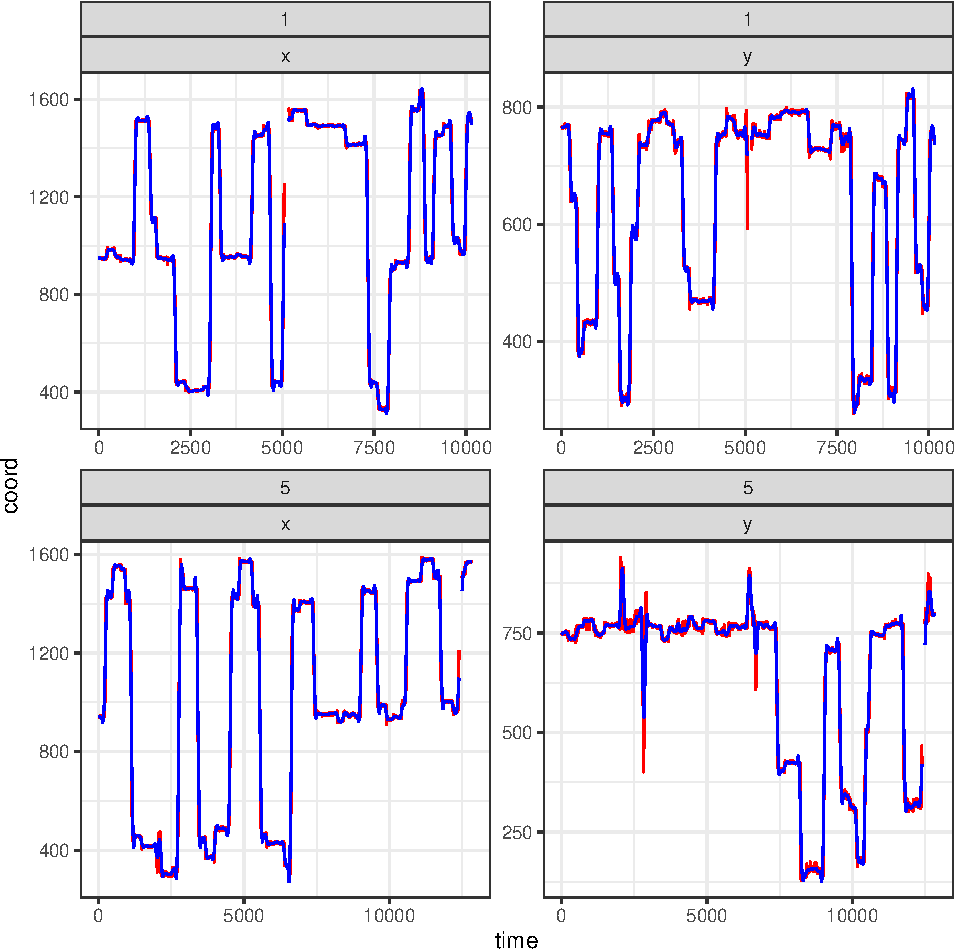
\includegraphics{BRM_ms_files/figure-pdf/unnamed-chunk-6-1.pdf}

\subsection{Fixations}\label{fixations}

Once the data has been repaired and smoothed, a core step in eye data
analysis is to identify fixations
(\citeproc{ref-salvucci2000identifying}{Salvucci \& Goldberg, 2000}),
defined as when the gaze stops in a specific location for a given amount
of time. When the eyes are moving between these fixations, they are
considered to be saccades. Subsequently, data can be split into these
two groups, fixations and saccades. In the eyetools package, there are
two fixation algorithms offered; the first algorithm,
\texttt{fixation\_dispersion()} employs a dispersion-based approach that
uses spatial and temporal data to determine fixations. By using a
maximum dispersion range, the algorithm looks for sufficient periods of
time that the eye gaze remains within this range and once this range is
exceed, this is termed as a fixation. The second algorithm,
\texttt{fixation\_VTI()} takes advantage of the idea that data is either
a fixation or a saccade and employs a velocity-threshold approach. It
identifies data where the eye is moving at a minimum velocity and
excludes this, before applying a dispersion check to ensure that the eye
does not drift during the fixation period. If the range is broken, a new
fixation is determined. Saccades must be of a given length to be
removed, otherwise they are considered as micro-saccades
{[}@CITATION\_NEEDED\_HERE?{]}.

Additionally, in certain analyses it may be useful to extract the
saccades themselves. This can be achieved using the
\texttt{saccade\_VTI()} function.

Once fixations have been calculated, they can be used in conjunction
with Areas of Interest (AOIs) to determine the sequence in which the eye
enters and exits these areas, as well as the time spent in these
regions. When referring to AOIs, these often refer to the cues presented
and the outcome object. In our example, the two cues at the top of the
screen are the cues, and the outcome is at the bottom. We can define
these areas in a separate dataframe object by giving the centrepoint of
the AOI in x, y coordinates along with the width and height (if the AOIs
are rectangular) or just the radius (if circular).

In combination with the fixation data, the AOI information can be used
to determine the sequence of AOI entries using the \texttt{AOI\_seq()}
function. This fucntion checks whether a fixation is detected within an
AOI, and if not, it is dropped from the output, and then provides a list
of the sequence of AOI entries, along with start and end timestamps, and
the duration.

Time spent in AOIs can also be calculated from fixations or raw data
using the \texttt{AOI\_time()} function available. This calculates the
time spent in each AOI in each trial, based on the data type given, in
our case fixation data.

If choosing to work with the raw data, there is also the option of using
\texttt{AOI\_time\_binned()} which allows for the trials to be split
into bins of a given length, and the time spent in AOIs calculated as a
result.

\subsection{eyetool assumptions {[}I DON'T KNOW WHERE THIS SHOULD GO
JUST
YET{]}}\label{eyetool-assumptions-i-dont-know-where-this-should-go-just-yet}

As with any data processing or analysis, there are certain assumptions
made when developing the eyetools package. Some of these are built into
the package directly, either as errors or warnings, such as the
assumption that data is ordered by participant ID (if present) and
trial, and some are not built in because they would limit the
flexibility of the package functionality. One built-in assumption is the
handling of missing data. eyetools expects track loss to be represented
as NA within the data, and so any system that provides a different
convention for recording track loss needs to be changed prior to using
eyetools functions.

During development, eyetools was tested using data collected from a
Tobii Pro Spectrum eye tracker recording at 300Hz. Screen resolutions
were constant at 1080x1920 pixels, and the timestamps were recorded in
milliseconds. Whilst most of the functions were designed to work with
any hardware provided the data is formatted to eyetools expectations
(with the exception of \texttt{hdf5\_to\_df()} and
\texttt{hdf5\_get\_event()} as these convert Tobii data), as well as not
relying on specific frequencies or resolutions (either through the
function behaviour, or by supplying parameters for specificity),
eyetools has not been tested on a diverse set of datasets.

Some default behaviours are in-built, but are easily overrided such as
parameters for resolution in the plotting functions. Similarly
\texttt{saccade\_VTI()} and \texttt{fixation\_VTI()} were tested with
300Hz data. For these functions, as the frequency increases, the
relative saccadic velocities will be lower meaning that the thresholds
need to be reduced. This is important to note when working with data
that is not recorded at 300Hz. To circumvent the potential issue of
sample rates being an issue, by default functions that require a sample
rate will deduce the frequency from the data rather than needing it to
be specified.

\subsection{Visualisations made easy}\label{visualisations-made-easy}

When working with eye data, it can be beneficial for the researcher to
familiarise themselves with the dataset. Visualising the data through
graphics can help to identify meaningful patterns that are obscured when
relying on statisitical analyses alone
(\citeproc{ref-kabacoffActionThirdEdition2022}{Kabacoff, 2022}).
Graphics are also very effective at conveying information in a way that
is easily grasped by a diverse audience. eyetools offers a selection of
in-built plotting functions that work with data at most stages of
processing. These plots are designed to aid in the researcher's
processing and data analysis.

The \texttt{plot\_AOI\_growth()} function offers the representation of
how an individual (on a single trial) spends their time looking at the
different AOIs. This can be useful to see how AOIs are interacted with
over time, and this can be presented as either a cumulative over time,
or as a proportion of the time spent in the trial.

\begin{figure}[H]

\caption{\label{fig-growth}Examples of the absolute and proportional
time plots from \texttt{plot\_AOI\_growth()}}

\begin{minipage}{0.50\linewidth}

\subcaption{\label{fig-abs}}

\centering{

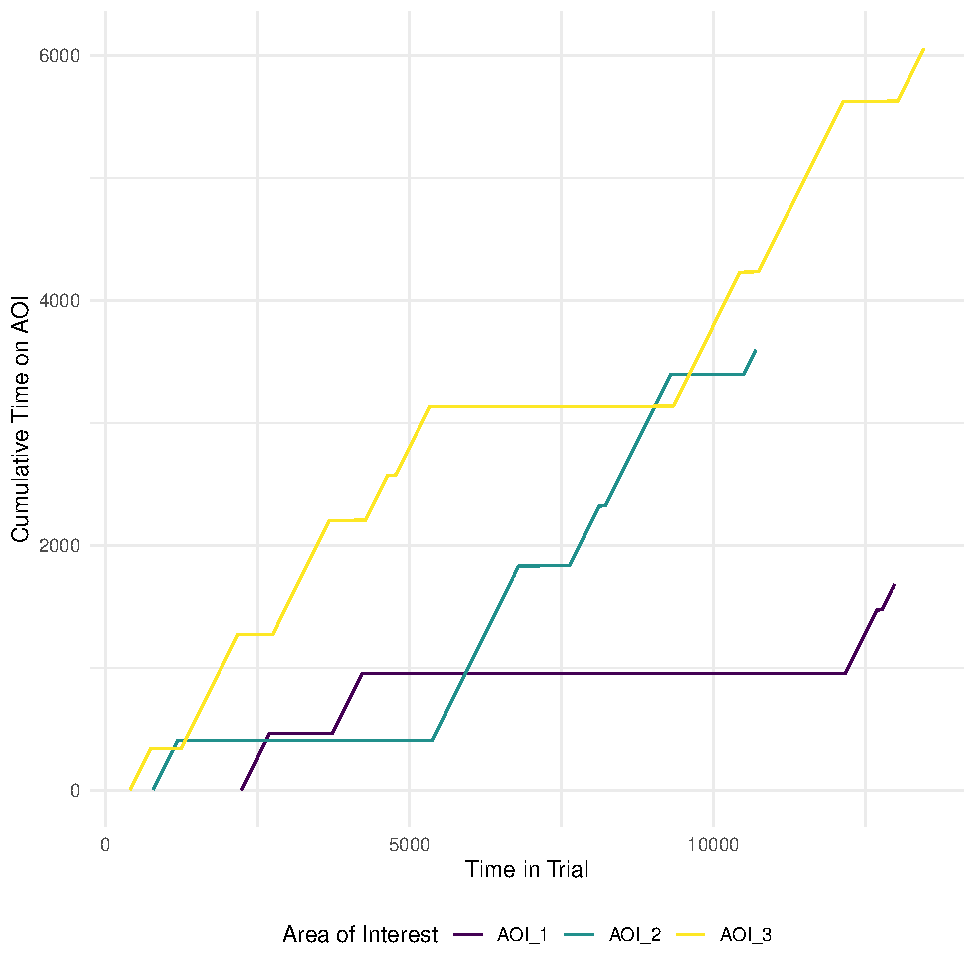
\includegraphics{BRM_ms_files/figure-pdf/fig-abs-1.pdf}

}

\end{minipage}%
%
\begin{minipage}{0.50\linewidth}

\subcaption{\label{fig-prop}}

\centering{

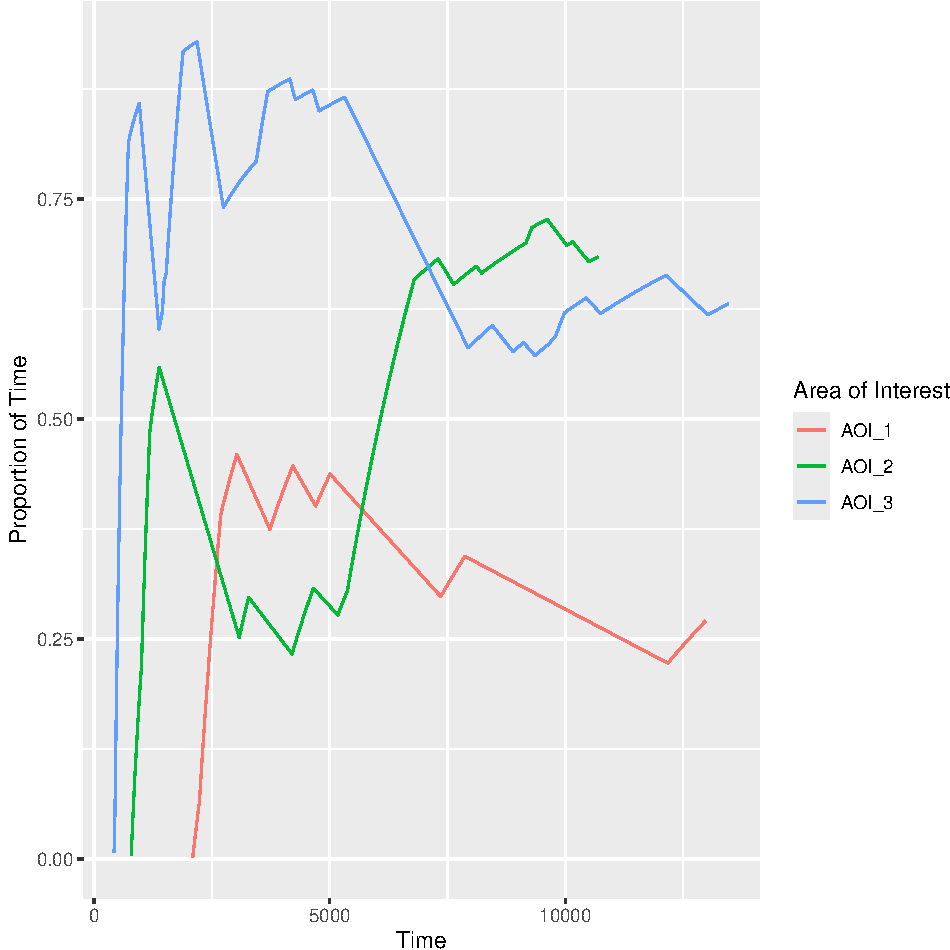
\includegraphics{BRM_ms_files/figure-pdf/fig-prop-1.pdf}

}

\end{minipage}%

\end{figure}%

A heatmap of eye gaze positions can be generated using
\texttt{plot\_heatmap()} which takes raw data as an input. As a
function, and unlike many of the processing steps, it does not
differentiate between trials or participants and plots any coordinate
data it is given. This behaviour is allowed as the heatmap offers an
excellent and fast ``sanity check'' that participants were, on the
whole, looking at the expected areas of the experiment screen during the
trials. As can be seen in Figure Figure~\ref{fig-heatmap}, we can be
reassured that participants do indeed spend most of their time looking
at the stimuli on screen rather than in the empty space.
\texttt{plot\_heatmap()} also allows for the modification of the amount
of data displayed, using the \texttt{alpha\_control} parameter. By
decreasing \texttt{alpha\_control} in Figure
Figure~\ref{fig-heatmap-alpha-update}, we gain more visualised
information and we can still see that the majority of the data is kept
within the stimuli and saccades between these areas.

\begin{figure}[H]

\caption{\label{fig-heatmap}A heatmap overlaid upon a sample stimuli
image demonstrating where the participants looked most over all trials}

\centering{

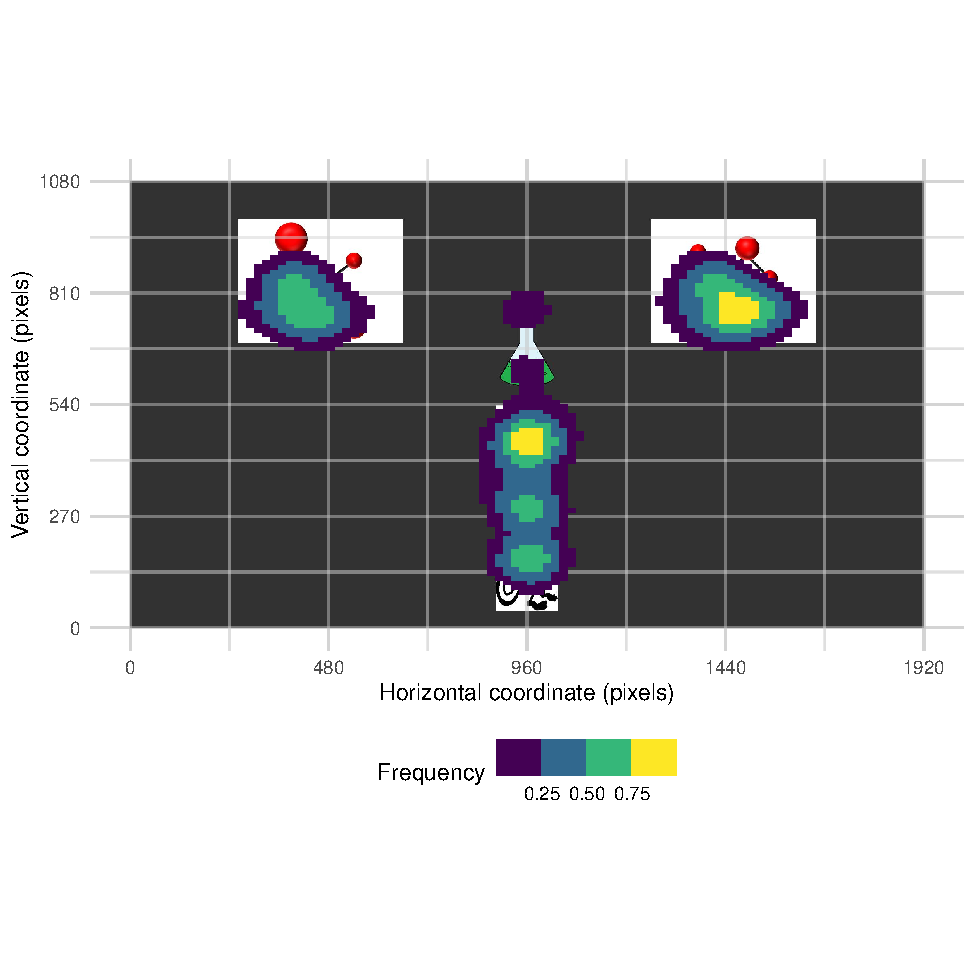
\includegraphics{BRM_ms_files/figure-pdf/fig-heatmap-1.pdf}

}

\end{figure}%

\begin{figure}[H]

\caption{\label{fig-heatmap-alpha-update}A heatmap overlaid upon a
sample stimuli image demonstrating where the participants looked most
over all trials}

\centering{

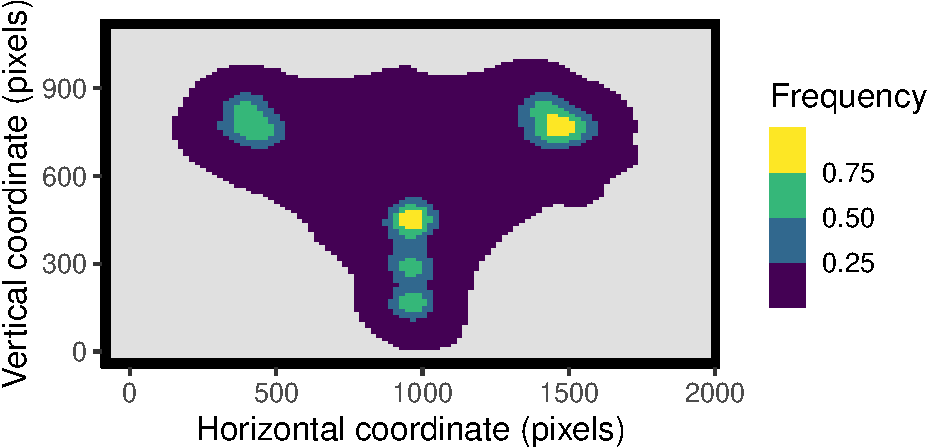
\includegraphics{BRM_ms_files/figure-pdf/fig-heatmap-alpha-update-1.pdf}

}

\end{figure}%

The \texttt{plot\_seq()} function allows for the plotting of raw data to
visualise the gaze pattern from a single trial and where the gaze fell
on the screen across the entire trial. Figure~\ref{fig-seq} offers an
example trial split into time bins of 5000ms. This plot shows the time
dimension as a change in colour that overlaps older data. This plot
serves as a useful check, similar to \texttt{plot\_heatmap()}, as to
where the eyes spent their time, but \texttt{plot\_seq()} has the
benefit of showing the time dimension compared to a simple heatmap.

\begin{figure}[H]

\caption{\label{fig-seq}The output from plot\_seq() with included AOIs
and time binned into 5 second sections}

\centering{

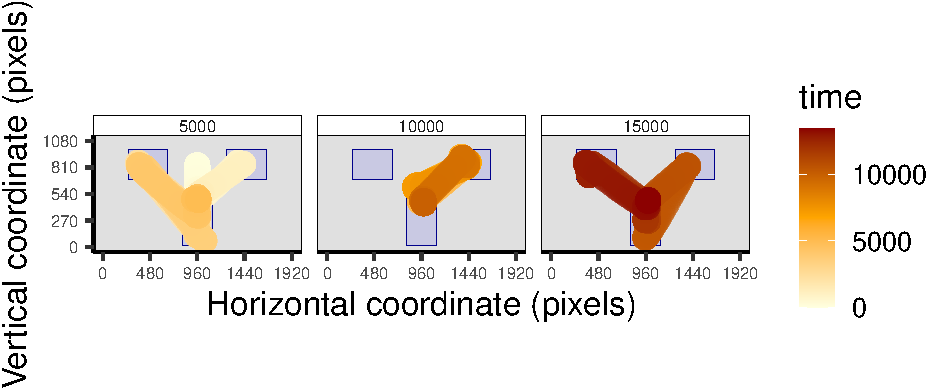
\includegraphics{BRM_ms_files/figure-pdf/fig-seq-1.pdf}

}

\end{figure}%

The final plotting function in eyetools is \texttt{plot\_spatial()}.
This can plot raw data, fixations, and saccades, either separately or in
combination. \texttt{plot\_spatial()} plots the location of the eye gaze
of a trial, and when given raw data is very similar to the output of
\texttt{plot\_seq()}, when using fixation data, then an additional
parameter can be used to label the fixations in their temporal order,
enabling a better presentation of how fixations arise. Finally,
providing saccade data allows for the length and direction of saccades
to be presented.

\begin{figure}[H]

\caption{\label{fig-spatial}The three types of plot that can be created
using \texttt{plot\_spatial()}}

\begin{minipage}{0.33\linewidth}

\subcaption{\label{fig-spatial-raw}}

\centering{

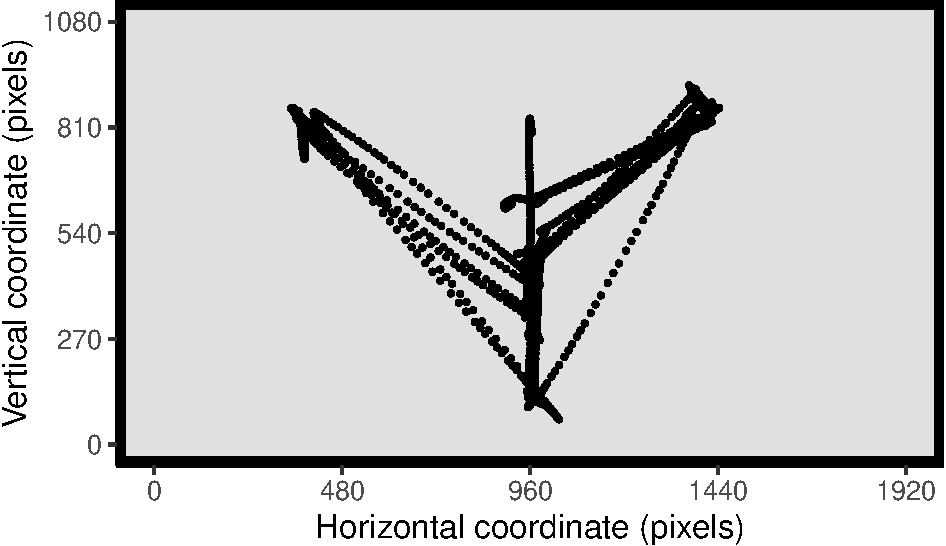
\includegraphics{BRM_ms_files/figure-pdf/fig-spatial-raw-1.pdf}

}

\end{minipage}%
%
\begin{minipage}{0.33\linewidth}

\subcaption{\label{fig-spatial-fix}}

\centering{

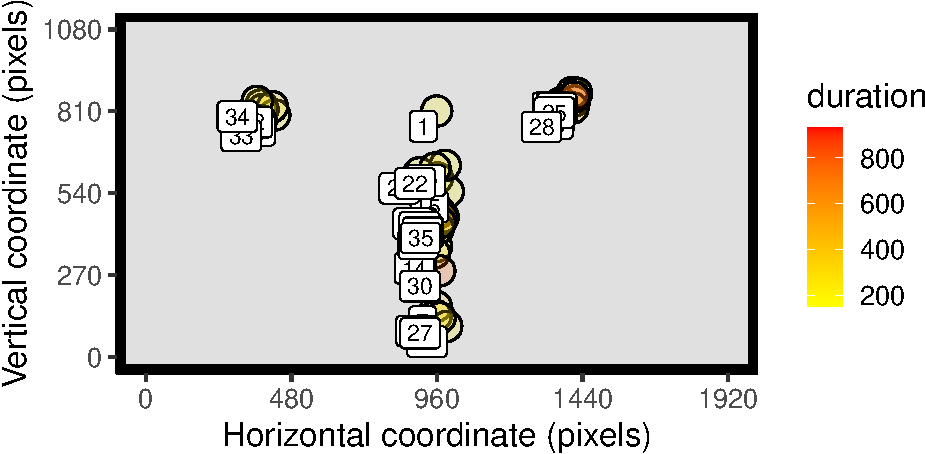
\includegraphics{BRM_ms_files/figure-pdf/fig-spatial-fix-1.pdf}

}

\end{minipage}%
%
\begin{minipage}{0.33\linewidth}

\subcaption{\label{fig-spatial-sac}}

\centering{

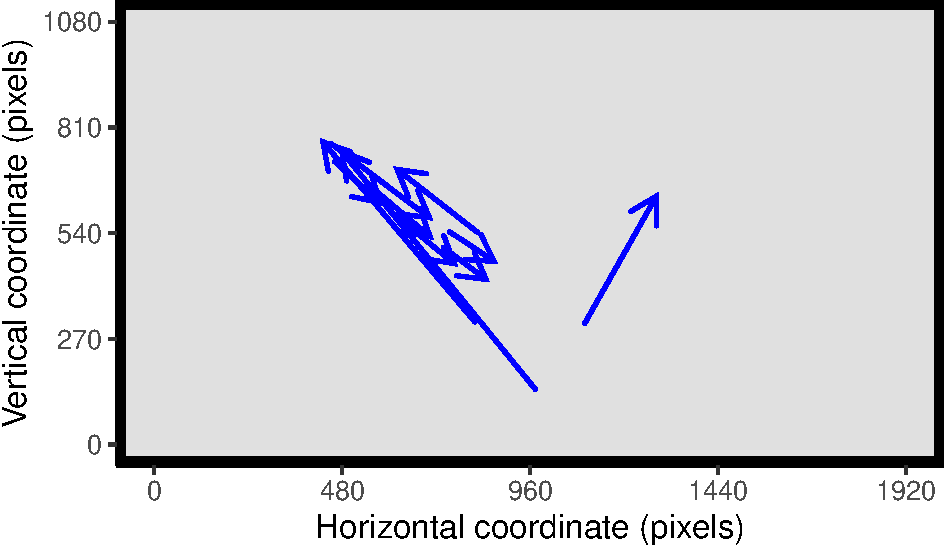
\includegraphics{BRM_ms_files/figure-pdf/fig-spatial-sac-1.pdf}

}

\end{minipage}%

\end{figure}%

\section{Analysing eye data}\label{analysing-eye-data}

@tom

\section{Discussion}\label{discussion}

In the present tutorial, we began by identifying the current gap in
available tools for working with eye data in open-science pipelines. We
then provided an overview of the general data collection process
required for eye tracking research, before detailing the conversion of
raw eye data into a useable eyetools format. We then covered the entire
processing pipeline using functions available in the eyetools package
that included the repairing and normalising the data, and the detection
of events such as fixations, saccades, and AOI entries.
@SOMETHING\_ON\_THE\_ANALYSIS\_GOES\_HERE.

From a practical perspective, this tutorial offers a step-by-step
walkthrough for handling eye data using R for open-science, reproducible
purposes. It provides a pipeline that can be relied upon by novices
looking to work with eye data, as well as offering new functions and
tools for experienced researchers. By enabling the processing and
analysis of data in a single R environment it also helps to speed up
data analysis.

\subsection{Advantages of Open-Source
Tools}\label{advantages-of-open-source-tools}

eyetools offers an open-source toolset that holds no hidden nor
proprietary functionality. The major benefits of open-source tools are
extensive, but the main ones include the ability to explore and engage
with the underlying functions to ensure that

A collaborative community - with open source tools, if an unmet need is
identified, then the community can work to provide a solution.

\subsection{Good Science Practices with
eyetools}\label{good-science-practices-with-eyetools}

Creating savepoints (like having processed raw data, and then
post-fixation calculation). Reduces the need to completely rework
workflows if an issue is detected as savepoints can be used to ensure
that computationally-intense or time-heavy processes are conducted as
infrequently as possible.

\section{Data Availability}\label{data-availability}

The data required for reproducing this tutorial is available at: @URL. A
condensed version of the dataset (starting with the
\texttt{combine\_eyes()} function) is a dataset in the eyetools package
called HCL.

\section{Code Availability}\label{code-availability}

The code used in this tutorial is available in the reproducible
manuscript file available at:(IF STORING IN GITHUB, THEN WE NEED TO
CREATE A ZENODO SNAPSHOT FOR A DOI RATHER THAN JUST A GITHUB LINK)

\section{References}\label{references}

\phantomsection\label{refs}
\begin{CSLReferences}{1}{0}
\bibitem[\citeproctext]{ref-duchowski2017eye}
Duchowski, A. T., \& Duchowski, A. T. (2017). \emph{Eye tracking
methodology: Theory and practice}. Springer.

\bibitem[\citeproctext]{ref-kabacoffActionThirdEdition2022}
Kabacoff, R. I. (2022). \emph{R in action: Data analysis and graphics
with r and tidyverse}. Simon; Schuster.

\bibitem[\citeproctext]{ref-salvucci2000identifying}
Salvucci, D. D., \& Goldberg, J. H. (2000). Identifying fixations and
saccades in eye-tracking protocols. \emph{Proceedings of the 2000
Symposium on Eye Tracking Research \& Applications}, 71--78.

\end{CSLReferences}






\end{document}
